\documentclass[tikz,border=2pt]{standalone}
\usepackage{amsmath}
\usepackage{pgfplots}
\pgfplotsset{compat=1.18}
\usetikzlibrary{arrows.meta}
\begin{document}
% x'' + 3x' + 2x = 4t: x_p = 2t - 3 and 2t - 3 + 2e^{-t} are both particular solutions; their difference
% 2e^{-t} solves the homogeneous equation (r = -1 is a root of r^2 + 3r + 2) and dies out.
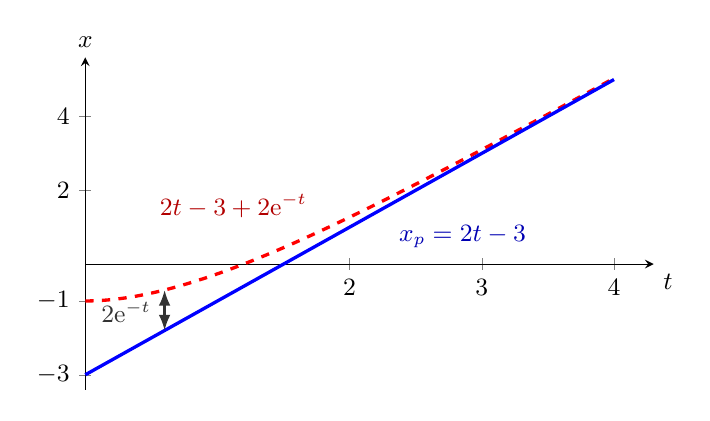
\begin{tikzpicture}[font=\small, >={Latex[length=2mm]}]
  \begin{axis}[
    axis lines=middle,
    xmin=0, xmax=4.3, ymin=-3.4, ymax=5.6,
    xtick={2,3,4}, ytick={-3,-1,2,4},
    xlabel={$t$}, ylabel={$x$},
    xlabel style={anchor=north west}, ylabel style={anchor=south},
    samples=100, clip=false,
    width=8.8cm, height=5.8cm
  ]
    \addplot[red, very thick, dashed, domain=0:4] {2*x-3+2*exp(-x)};
    \addplot[blue, very thick, domain=0:4] {2*x-3};
    % difference = homogeneous solution
    \draw[<->, gray!40!black, thick] (axis cs:0.6,-1.8) -- (axis cs:0.6,{-1.8+2*exp(-0.6)});
    \node[gray!40!black, anchor=east] at (axis cs:0.57,-1.3) {$2\mathrm{e}^{-t}$};
    \node[blue!70!black, anchor=north west] at (axis cs:2.3,1.3) {$x_p=2t-3$};
    \node[red!70!black, anchor=south east] at (axis cs:1.75,1.0) {$2t-3+2\mathrm{e}^{-t}$};
  \end{axis}
\end{tikzpicture}
\end{document}
